\documentclass[landscape]{slides}
\usepackage{url}
\usepackage{amsmath}
\usepackage{graphicx}
\usepackage{color}
\usepackage{epic,ecltree}
%\usepackage{bar}
\usepackage{eclbip}
\usepackage{array}
\usepackage{algorithmic}
\usepackage{algorithm}
\renewcommand{\algorithmicrequire}{\textbf{Input:}}
\renewcommand{\algorithmicensure}{\textbf{Output:}}
\renewcommand{\algorithmiccomment}[1]{// {\em #1}}

\definecolor{darkblue}{rgb}{0,0,0.8}
\definecolor{darkgreen}{rgb}{0,0.8,0}
\definecolor{purple}{rgb}{0.6,0,0.6}
\definecolor{red}{rgb}{1,0,0}

\newcommand{\example}[1]{\textcolor{darkblue}{\rm #1}}
\newcommand{\maths}[1]{\textcolor{purple}{#1}}
\newcommand{\reference}[1]{\vspace{-2mm}\begin{flushright}\textcolor{purple}{\tiny [from #1]}\end{flushright}\vspace{-7mm}}

\begin{document}
\title[Chapter 6: Decoding]{Chapter 6\\[1cm] Decoding}
\author[Philipp Koehn]{}
\date{Statistical Machine Translation}

\maketitle

%%%%%%%%%%%%%%%%%%%%%%%%%%%%%%%%%%%%%%%%%%%%%%%%%%%%%%%%%%%%%%%%%%%%%%%%%%%%

\slide{Decoding}
\begin{itemize}
\item We have a mathematical model for translation \vspace{-5mm}
\maths{\begin{equation*}
p({\bf e}|{\bf f})\vspace{-20mm}
\end{equation*}}
\item Task of decoding: find the translation \maths{${\bf e}_\text{best}$} with highest probability\vspace{-5mm}
\maths{\begin{equation*}
{\bf e}_\text{best} = \text{argmax}_{\bf e} \; p({\bf e}|{\bf f})\vspace{-20mm}
\end{equation*}}
\item Two types of error
\begin{itemize}
\item the most probable translation is bad $\rightarrow$ fix the model
\item search does not find the most probably translation $\rightarrow$ fix the search
\end{itemize}
\item Decoding is evaluated by search error, not quality of translations\\
(although these are often correlated)
\end{itemize}

%%%%%%%%%%%%%%%%%%%%%%%%%%%%%%%%%%%%%%%%%%%%%%%%%%%%%%%%%%%%%%%%%%%%%%%%%%%

\slide{Translation Process}
\begin{itemize} \vspace{10mm}
\item Task: translate this sentence from German into English\vspace{4mm}
\end{itemize} 
\begin{center}
$\;$ $\;$ $\;\;$ 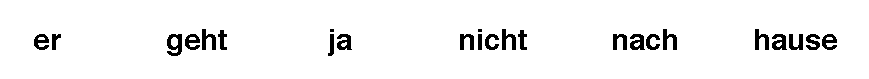
\includegraphics[scale=1.5]{translation-step1.pdf}
\end{center}

%%%%%%%%%%%%%%%%%%%%%%%%%%%%%%%%%%%%%%%%%%%%%%%%%%%%%%%%%%%%%%%%%%%%%%%%%%%%

\slide{Translation  Process}
\begin{itemize} \vspace{10mm}
\item Task: translate this sentence from German into English
\begin{center}
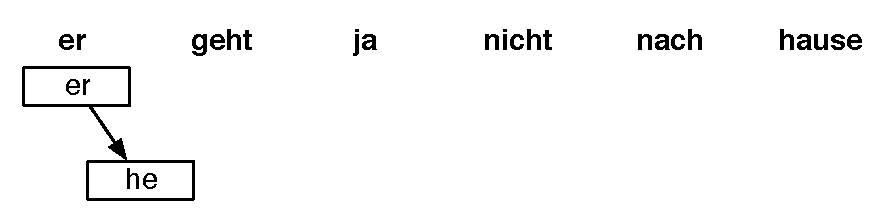
\includegraphics[scale=1.5]{translation-step2.pdf}
\end{center}
\item Pick phrase in input, translate
\end{itemize}


%%%%%%%%%%%%%%%%%%%%%%%%%%%%%%%%%%%%%%%%%%%%%%%%%%%%%%%%%%%%%%%%%%%%%%%%%%%%%

\slide{Translation  Process}
\begin{itemize}\vspace{10mm}
\item Task: translate this sentence from German into English
\begin{center}
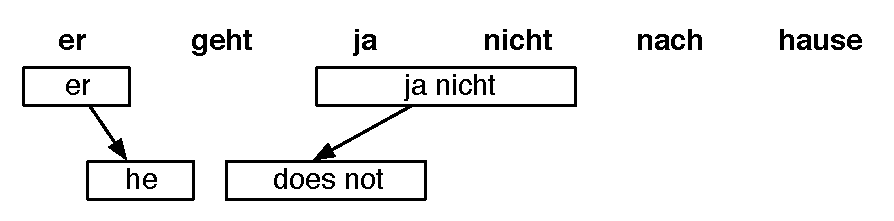
\includegraphics[scale=1.5]{translation-step3.pdf}
\end{center}
\item Pick phrase in input, translate
\begin{itemize}
\item it is allowed to pick words out of sequence reordering
\item phrases may have multiple words: many-to-many translation
\end{itemize}
\end{itemize}

%%%%%%%%%%%%%%%%%%%%%%%%%%%%%%%%%%%%%%%%%%%%%%%%%%%%%%%%%%%%%%%%%%%%%%%%%%%%%

\slide{Translation  Process}
\begin{itemize}\vspace{10mm}
\item Task: translate this sentence from German into English
\begin{center}
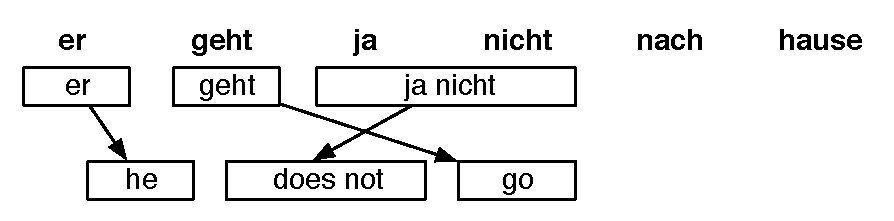
\includegraphics[scale=1.5]{translation-step4.pdf}
\end{center}
\item Pick phrase in input, translate
\end{itemize}

%%%%%%%%%%%%%%%%%%%%%%%%%%%%%%%%%%%%%%%%%%%%%%%%%%%%%%%%%%%%%%%%%%%%%%%%%%%%

\slide{Translation  Process}
\begin{itemize}\vspace{10mm}
\item Task: translate this sentence from German into English
\begin{center}
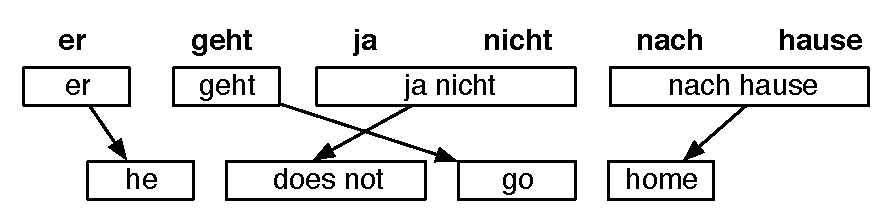
\includegraphics[scale=1.5]{translation-step5.pdf}
\end{center}
\item Pick phrase in input, translate
\end{itemize}

%%%%%%%%%%%%%%%%%%%%%%%%%%%%%%%%%%%%%%%%%%%%%%%%%%%%%%%%%%%%%%%%%%%%%%%%%%%%

\slide{Computing Translation Probability}
\begin{itemize}
\item Probabilistic model for phrase-based translation:
\maths{\begin{equation*}
{\bf e}_{\mbox{\small best}} = \text{argmax}_{\bf e} \; \prod_{i=1}^I \phi(\bar{f}_i|\bar{e}_i) \; d(start_i-end_{i-1}-1) \; p_{\text{\sc lm}}({\bf e})
\end{equation*}} \vspace{-10mm}
\item Score is computed incrementally for each partial hypothesis
\item Components
\begin{description}
\item[{\bf Phrase translation}] Picking phrase \maths{$\bar{f_i}$} to be translated as a phrase \maths{$\bar{e_i}$}\\ $\rightarrow$ look up score \maths{$\phi(\bar{f}_i|\bar{e}_i)$} from phrase translation table
\item[{\bf Reordering}] Previous phrase ended in \maths{$end_{i-1}$}, current phrase starts at \maths{$start_i$}\\  $\rightarrow$ compute \maths{$d(start_i-end_{i-1}-1)$}
\item[{\bf Language model}] For \maths{$n$}-gram model, need to keep track of last \maths{$n-1$} words\\  $\rightarrow$ compute score \maths{$p_\text{\sc lm}(w_i|w_{i-(n-1)}, ..., w_{i-1})$} for added words \maths{$w_i$}
\end{description}
\end{itemize}

%%%%%%%%%%%%%%%%%%%%%%%%%%%%%%%%%%%%%%%%%%%%%%%%%%%%%%%%%%%%%%%%%%%%%%%%%%%%%

\slide{Translation Options}
\begin{center} 
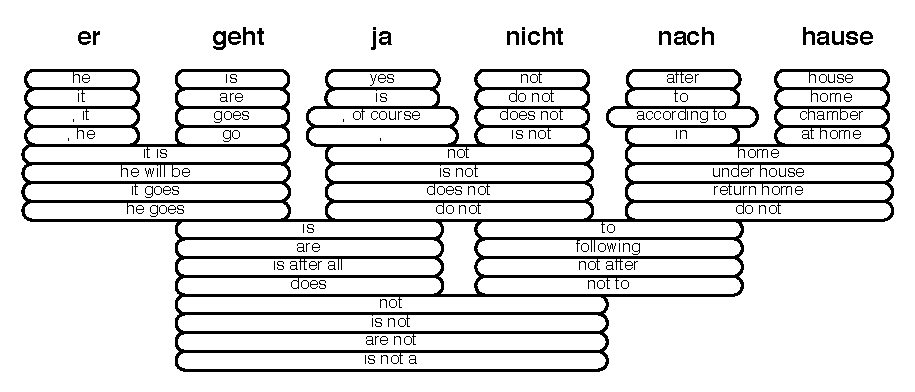
\includegraphics[scale=1.5]{translation-options.pdf}
\end{center}\vspace{-10mm}
\begin{itemize}
\item Many translation options to choose from
\begin{itemize} \vspace{-1mm}
\item in Europarl phrase table: 2727 matching phrase pairs for this sentence
\item by pruning to the top 20 per phrase, 202 translation options remain
\end{itemize}
\end{itemize}

%%%%%%%%%%%%%%%%%%%%%%%%%%%%%%%%%%%%%%%%%%%%%%%%%%%%%%%%%%%%%%%%%%%%%%%%%%%%%

\slide{Translation Options}
\begin{center} 
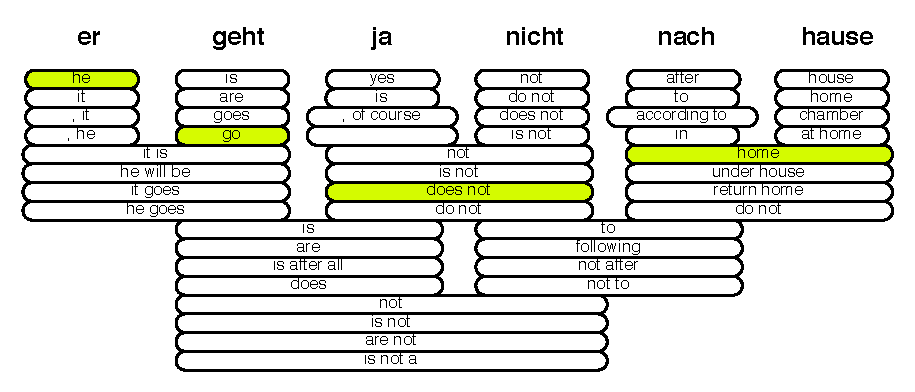
\includegraphics[scale=1.5]{translation-options-correct.pdf}
\end{center}  \vspace{-10mm}
\begin{itemize}
\item The machine translation decoder does not know the right answer\vspace{-4mm}
\begin{itemize}
\item picking the right translation options
\item arranging them in the right order \vspace{-4mm}
\end{itemize}
\item[$\rightarrow$] Search problem solved by heuristic beam search
\end{itemize}

%%%%%%%%%%%%%%%%%%%%%%%%%%%%%%%%%%%%%%%%%%%%%%%%%%%%%%%%%%%%%%%%%%%%%%%%%%%%%

\slide{Decoding: Precompute Translation Options}
\begin{center}
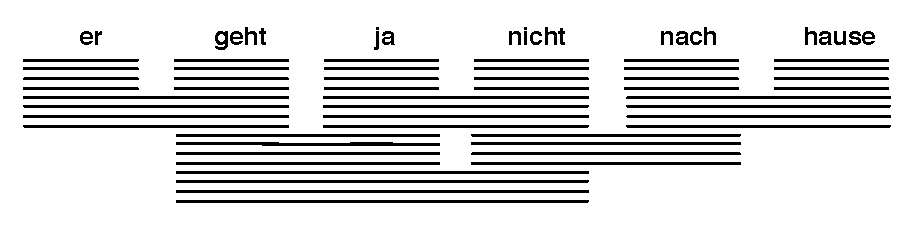
\includegraphics[scale=1.3]{decoding-step1.pdf}\\[69mm]
consult phrase translation table for all input phrases
\end{center}

%%%%%%%%%%%%%%%%%%%%%%%%%%%%%%%%%%%%%%%%%%%%%%%%%%%%%%%%%%%%%%%%%%%%%%%%%%%%

\slide{Decoding: Start with Initial Hypothesis}
\begin{center} 
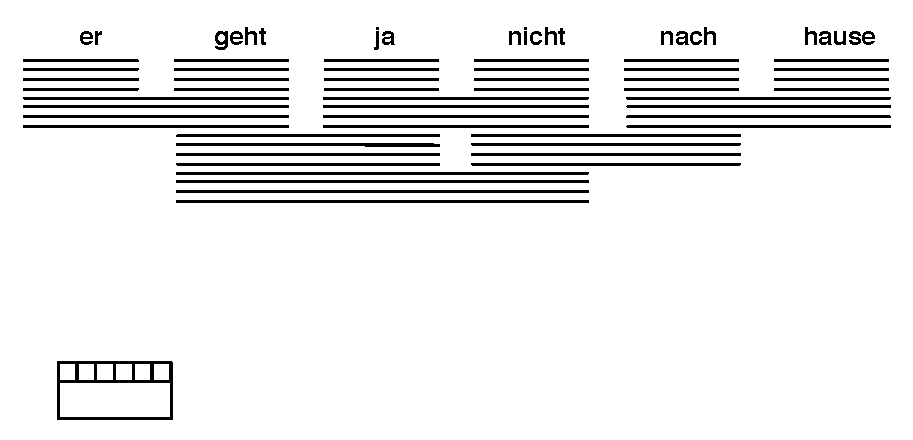
\includegraphics[scale=1.3]{decoding-step2.pdf}\\[22mm]
initial hypothesis: no input words covered, no output produced
\end{center}

%%%%%%%%%%%%%%%%%%%%%%%%%%%%%%%%%%%%%%%%%%%%%%%%%%%%%%%%%%%%%%%%%%%%%%%%%%%%

\slide{Decoding: Hypothesis Expansion}
\begin{center}
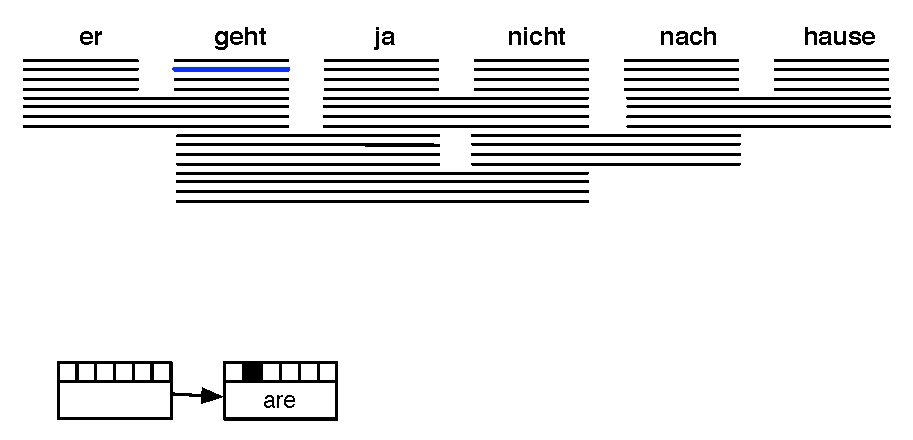
\includegraphics[scale=1.3]{decoding-step3.pdf}\\[22mm]
pick any translation option, create new hypothesis
\end{center} 

%%%%%%%%%%%%%%%%%%%%%%%%%%%%%%%%%%%%%%%%%%%%%%%%%%%%%%%%%%%%%%%%%%%%%%%%%%%%

\slide{Decoding: Hypothesis Expansion}
\begin{center} 
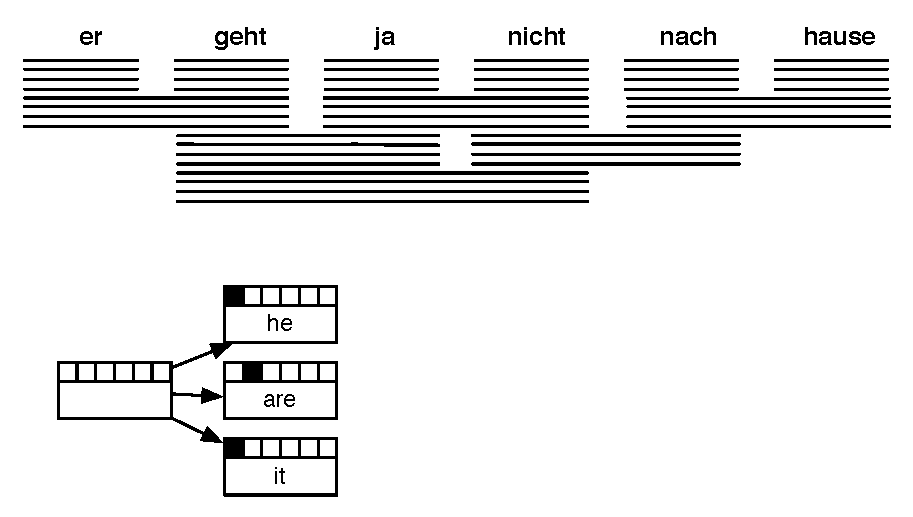
\includegraphics[scale=1.3]{decoding-step4.pdf}\\[5mm]
create hypotheses for all other translation options
\end{center}

%%%%%%%%%%%%%%%%%%%%%%%%%%%%%%%%%%%%%%%%%%%%%%%%%%%%%%%%%%%%%%%%%%%%%%%%%%%%

\slide{Decoding: Hypothesis Expansion}
\begin{center} 
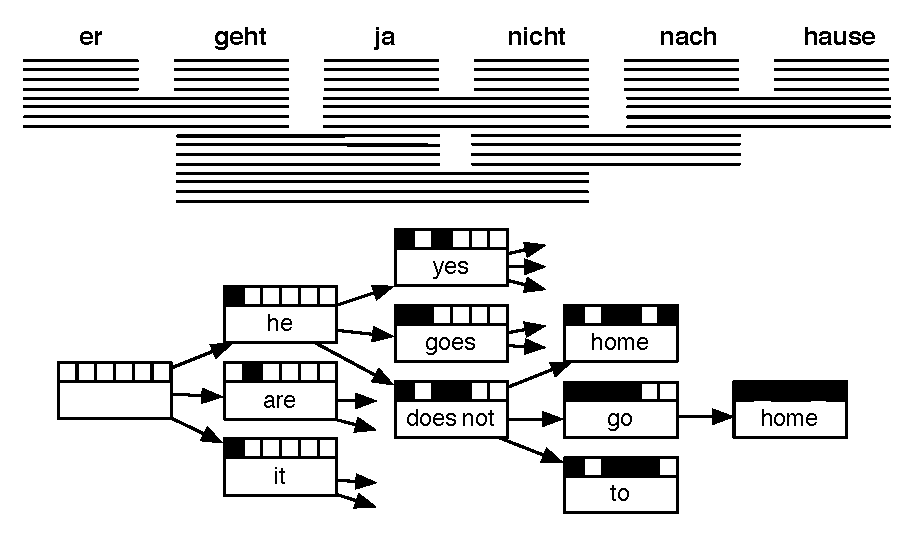
\includegraphics[scale=1.3]{decoding-step5.pdf}\\
also create hypotheses from created partial hypothesis
\end{center}

%%%%%%%%%%%%%%%%%%%%%%%%%%%%%%%%%%%%%%%%%%%%%%%%%%%%%%%%%%%%%%%%%%%%%%%%%%%%

\slide{Decoding: Find Best Path}
\begin{center}
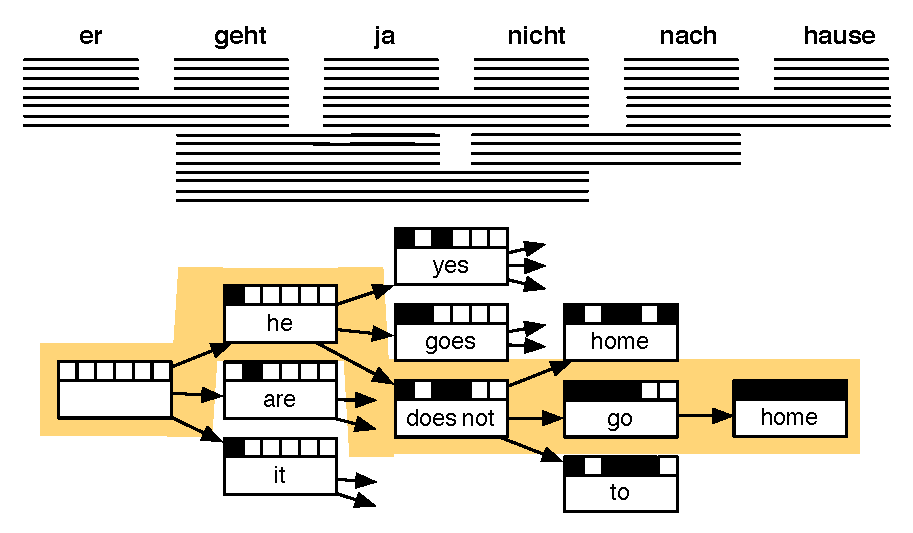
\includegraphics[scale=1.3]{decoding-step6.pdf}\\[1mm]
backtrack from highest scoring complete hypothesis
\end{center}

%%%%%%%%%%%%%%%%%%%%%%%%%%%%%%%%%%%%%%%%%%%%%%%%%%%%%%%%%%%%%%%%%%%%%%%%%%%%

\slide{Computational Complexity}
\begin{itemize}\vspace{25mm}
\item The suggested process creates exponential number of hypothesis 
\item Machine translation decoding is NP-complete
\item Reduction of search space:
\begin{itemize}
\item recombination (risk-free)
\item pruning (risky)
\end{itemize}
\end{itemize}

%%%%%%%%%%%%%%%%%%%%%%%%%%%%%%%%%%%%%%%%%%%%%%%%%%%%%%%%%%%%%%%%%%%%%%%%%%%%

\slide{Recombination}
\begin{itemize}
\item Two hypothesis paths lead to two matching hypotheses
\begin{itemize}
\item same number of foreign words translated
\item same English words in the output
\item different scores
\end{itemize}
\begin{center} \vspace{-10mm}
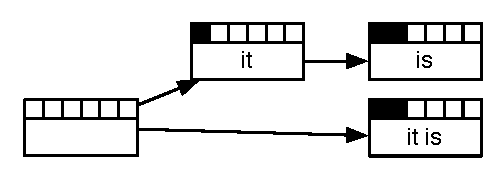
\includegraphics[scale=1.3]{recombination-example1.pdf}
\end{center}
\item  Worse hypothesis is dropped
\begin{center} \vspace{-5mm}
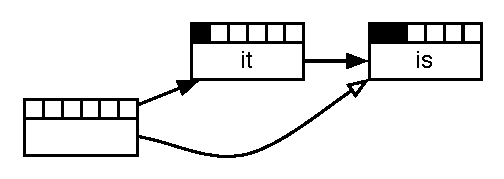
\includegraphics[scale=1.3]{recombination-example2.pdf}
\end{center}
\end{itemize}

%%%%%%%%%%%%%%%%%%%%%%%%%%%%%%%%%%%%%%%%%%%%%%%%%%%%%%%%%%%%%%%%%%%%%%%%%%%%

\slide{Recombination}
\begin{itemize}
\item Two hypothesis paths lead to hypotheses indistinguishable in subsequent search
\begin{itemize}
\item same number of foreign words translated
\item same last two English words in output (assuming trigram language model)
\item same last foreign word translated
\item different scores
\end{itemize}\vspace{-10mm}
\begin{center}
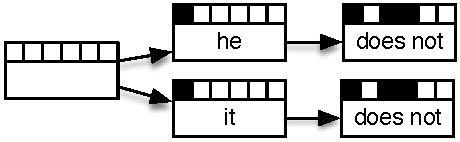
\includegraphics[scale=1.3]{recombination-example3b.pdf}
\end{center}\vspace{-12mm}
\item  Worse hypothesis is dropped
\begin{center}\vspace{-7mm}
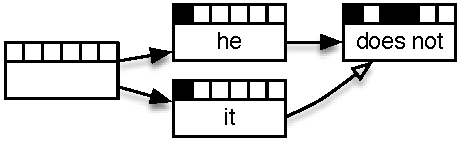
\includegraphics[scale=1.3]{recombination-example4b.pdf}
\end{center}
\end{itemize}

%%%%%%%%%%%%%%%%%%%%%%%%%%%%%%%%%%%%%%%%%%%%%%%%%%%%%%%%%%%%%%%%%%%%%%%%%%%%

\slide{Restrictions on Recombination}
\begin{itemize}\vspace{10mm}
\item {\bf Translation model:} Phrase translation independent from each other\\[3mm]
$\rightarrow$ no restriction to hypothesis recombination
\item {\bf Language model:} Last \maths{$n-1$} words used as history in \maths{$n$}-gram language model\\[3mm]
$\rightarrow$ recombined hypotheses must match in their last \maths{$n-1$} words
\item {\bf Reordering model:} Distance-based reordering model based on distance to end position of previous input phrase\\[3mm]
$\rightarrow$ recombined hypotheses must have that same end position
\item Other feature function may introduce additional restrictions
\end{itemize}


%%%%%%%%%%%%%%%%%%%%%%%%%%%%%%%%%%%%%%%%%%%%%%%%%%%%%%%%%%%%%%%%%%%%%%%%%%%%

\slide{Pruning}
\begin{itemize} \vspace{25mm}
\item Recombination reduces search space, but not enough\\[3mm]
(we still have a NP complete problem on our hands)
\item Pruning: remove bad hypotheses early
\begin{itemize}
\item put comparable hypothesis into stacks\\
(hypotheses that have translated same number of input words)
\item limit number of hypotheses in each stack
\end{itemize}
\end{itemize}

%%%%%%%%%%%%%%%%%%%%%%%%%%%%%%%%%%%%%%%%%%%%%%%%%%%%%%%%%%%%%%%%%%%%%%%%%%%%

\slide{Stacks}
\begin{center}
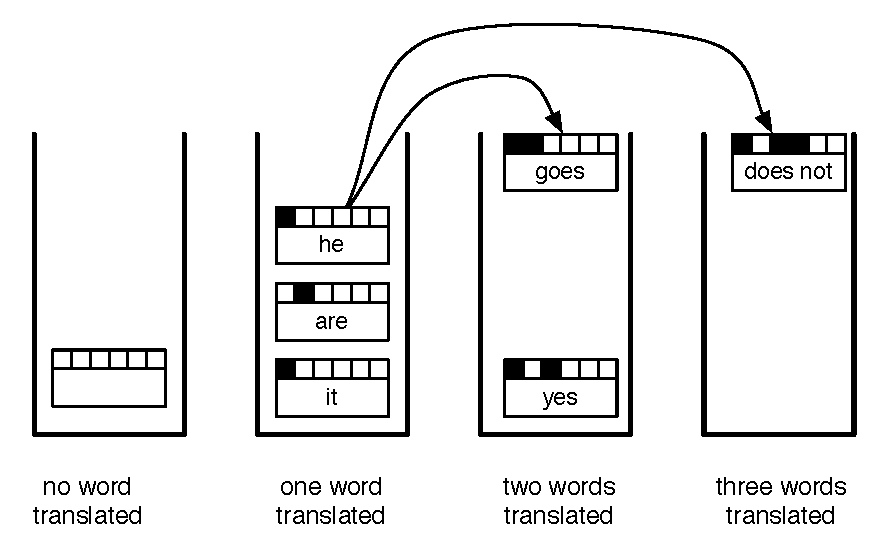
\includegraphics[scale=1.2]{hypothesis-stacks-fw.pdf}
\end{center} \vspace{-9mm}
\begin{itemize}
\item Hypothesis expansion in a stack decoder \vspace{-3mm}
\begin{itemize}
\item translation option is applied to hypothesis
\item new hypothesis is dropped into a stack further down
\end{itemize}
\end{itemize}

%%%%%%%%%%%%%%%%%%%%%%%%%%%%%%%%%%%%%%%%%%%%%%%%%%%%%%%%%%%%%%%%%%%%%%%%%%%%

\slide{Stack Decoding Algorithm}
\vspace{5mm}
\begin{tabular}{p{3cm}p{20cm}}
& \begin{algorithmic}[1]
\STATE place empty hypothesis into stack 0
\FORALL{stacks 0...$n-1$}
%  \STATE prune stack {\bf if} too big
  \FORALL{hypotheses in stack}
    \FORALL{translation options}
      \IF{applicable}
        \STATE create new hypothesis
        \STATE place in stack
        \STATE recombine with existing hypothesis {\bf if} possible
        \STATE prune stack {\bf if} too big
      \ENDIF
    \ENDFOR
  \ENDFOR
\ENDFOR 
\end{algorithmic}
\end{tabular}

%%%%%%%%%%%%%%%%%%%%%%%%%%%%%%%%%%%%%%%%%%%%%%%%%%%%%%%%%%%%%%%%%%%%%%%%%%%%

\slide{Pruning}
\begin{itemize}
\item Pruning strategies
\begin{itemize}
\item histogram pruning: keep at most \maths{$k$} hypotheses in each stack
\item stack pruning: keep hypothesis with score \maths{$\alpha$} $\times$ best score (\maths{$\alpha<1$})
\end{itemize}
\item Computational time complexity of decoding with histogram pruning
\maths{\begin{equation*}
O(\text{max stack size} \times \text{translation options} \times \text{sentence length})\vspace{-20mm}
\end{equation*}}
\item Number of translation options is linear with sentence length, hence:
\maths{\begin{equation*}
O(\text{max stack size} \times \text{sentence length}^2)\vspace{-20mm}
\end{equation*}}
\item Quadratic complexity
\end{itemize}

%%%%%%%%%%%%%%%%%%%%%%%%%%%%%%%%%%%%%%%%%%%%%%%%%%%%%%%%%%%%%%%%%%%%%%%%%%%%

\slide{Reordering Limits}
\begin{itemize}
\item Limiting reordering to maximum reordering distance
\item Typical reordering distance 5--8 words
\begin{itemize}
\item depending on language pair
\item larger reordering limit hurts translation quality
\end{itemize}
\item Reduces complexity to linear
\maths{\begin{equation*}
O(\text{max stack size} \times \text{sentence length})\vspace{-15mm}
\end{equation*}}
\item Speed / quality trade-off by setting maximum stack size
\end{itemize}

%%%%%%%%%%%%%%%%%%%%%%%%%%%%%%%%%%%%%%%%%%%%%%%%%%%%%%%%%%%%%%%%%%%%%%%%%%%%

\slide{Translating the Easy Part First?}
\begin{center} \vspace{10mm}
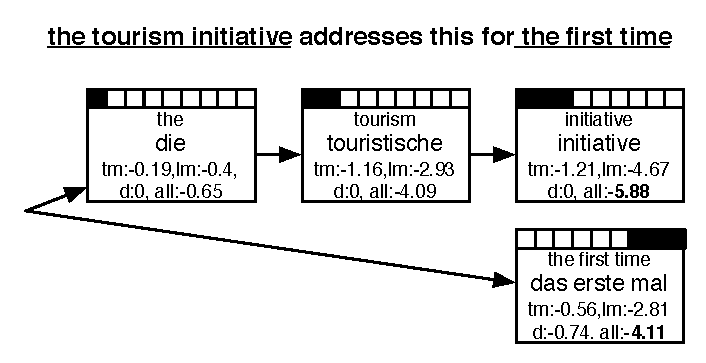
\includegraphics[scale=1.5]{hyp-cost-comparison.pdf}\\[10mm]
both hypotheses translate 3 words\\
worse hypothesis has better score
\end{center}

%%%%%%%%%%%%%%%%%%%%%%%%%%%%%%%%%%%%%%%%%%%%%%%%%%%%%%%%%%%%%%%%%%%%%%%%%%%%

\slide{Estimating Future Cost}
\begin{itemize}\vspace{10mm}
\item Future cost estimate: how expensive is translation of rest of sentence?
\item Optimistic: choose cheapest translation options
\item Cost for each translation option
\begin{itemize}
\item {\bf translation model}: cost known \vspace{4mm}
\item {\bf language model:} output words known, but not context\\ $\rightarrow$ estimate without context\vspace{4mm}
\item {\bf reordering model:} unknown, ignored for future cost estimation
\end{itemize}
\end{itemize}

%%%%%%%%%%%%%%%%%%%%%%%%%%%%%%%%%%%%%%%%%%%%%%%%%%%%%%%%%%%%%%%%%%%%%%%%%%%%

\slide{Cost Estimates from Translation Options}
\begin{center}
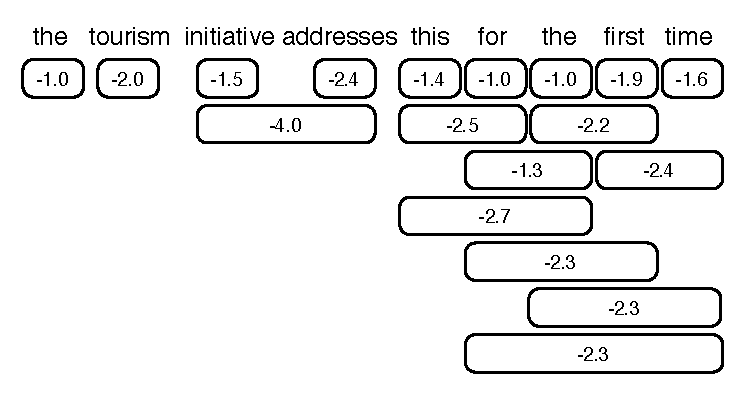
\includegraphics[scale=1.7]{future-cost-covered-spans.pdf}\\[8mm]
cost of cheapest translation options for each input span (log-probabilities)
\end{center}


%%%%%%%%%%%%%%%%%%%%%%%%%%%%%%%%%%%%%%%%%%%%%%%%%%%%%%%%%%%%%%%%%%%%%%%%%%%%

\slide{Cost Estimates for all Spans}
\begin{itemize} \vspace{-4mm}
\item Compute cost estimate for all contiguous spans by combining cheapest options\vspace{-2mm}
\begin{center}
\begin{tabular}{|c|c|c|c|c|c|c|c|c|c|c|} \hline
\bf first & \multicolumn{9}{c|}{\bf future cost estimate for $n$ words (from first)} \\ \cline{2-10}
\bf word & \bf 1 & \bf 2 & \bf 3 & \bf 4 & \bf 5 & \bf 6 & \bf 7 & \bf 8 & \bf 9 \\ \hline 
\example{the} & -1.0 &  -3.0 &  -4.5 &  -6.9 &  -8.3 &  -9.3 &  -9.6 & -10.6 & -10.6 \\ \hline
\example{tourism} & -2.0 &  -3.5 &  -5.9 &  -7.3 &  -8.3 &  -8.6 &  -9.6 &  -9.6 \\ \cline{1-9}
\example{initiative} & -1.5 &  -3.9 &  -5.3 &  -6.3 &  -6.6 &  -7.6 &  -7.6 \\\cline{1-8}
\example{addresses} & -2.4 &  -3.8 &  -4.8 &  -5.1 &  -6.1 &  -6.1 \\\cline{1-7}
\example{this} & -1.4 &  -2.4 &  -2.7 &  -3.7 &  -3.7 \\\cline{1-6}
\example{for} & -1.0 &  -1.3 &  -2.3 &  -2.3 \\\cline{1-5}
\example{the} & -1.0 &  -2.2 &  -2.3  \\\cline{1-4}
\example{first} & -1.9 &  -2.4  \\\cline{1-3}
\example{time} & -1.6  \\\cline{1-2}
\end{tabular}\vspace{-4mm}
\end{center} 
\item Function words cheaper (\example{the}: -1.0) than content words (\example{tourism} -2.0) \vspace{-8mm}
\item Common phrases cheaper (\example{for the first time}: -2.3)\\ than unusual ones (\example{tourism initiative addresses}: -5.9)
\end{itemize}

%%%%%%%%%%%%%%%%%%%%%%%%%%%%%%%%%%%%%%%%%%%%%%%%%%%%%%%%%%%%%%%%%%%%%%%%%%%%

\slide{Combining Score and Future Cost}
\begin{center}
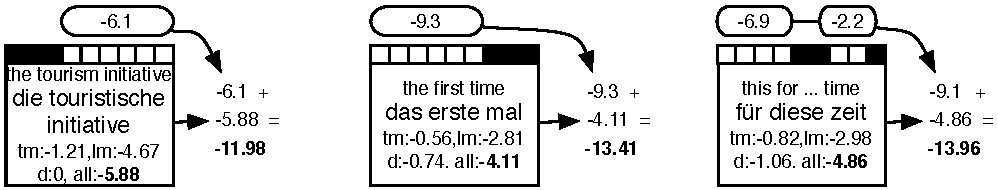
\includegraphics[scale=1.4]{future-cost-comparison.pdf}
\end{center}
\begin{itemize}
\item Hypothesis score and future cost estimate are combined for pruning
\begin{itemize}
\item left hypothesis starts with hard part: \example{the tourism initiative}\\
score: -5.88, future cost: -6.1 $\rightarrow$ total cost -11.98 \vspace{3mm}
\item middle hypothesis starts with easiest part: \example{the first time}\\
score: -4.11, future cost: -9.3 $\rightarrow$ total cost -13.41 \vspace{3mm}
\item right hypothesis picks easy parts: \example{this for ... time}\\
score: -4.86, future cost: -9.1 $\rightarrow$ total cost -13.96
\end{itemize}
\end{itemize}

%%%%%%%%%%%%%%%%%%%%%%%%%%%%%%%%%%%%%%%%%%%%%%%%%%%%%%%%%%%%%%%%%%%%%%%%%%%%

\slide{Other Decoding Algorithms}
\vspace{30mm}
\begin{itemize}
\item A* search
\item Greedy hill-climbing
\item Using finite state transducers (standard toolkits)
\end{itemize}

%%%%%%%%%%%%%%%%%%%%%%%%%%%%%%%%%%%%%%%%%%%%%%%%%%%%%%%%%%%%%%%%%%%%%%%%%%%%

\slide{A* Search}
\begin{center}
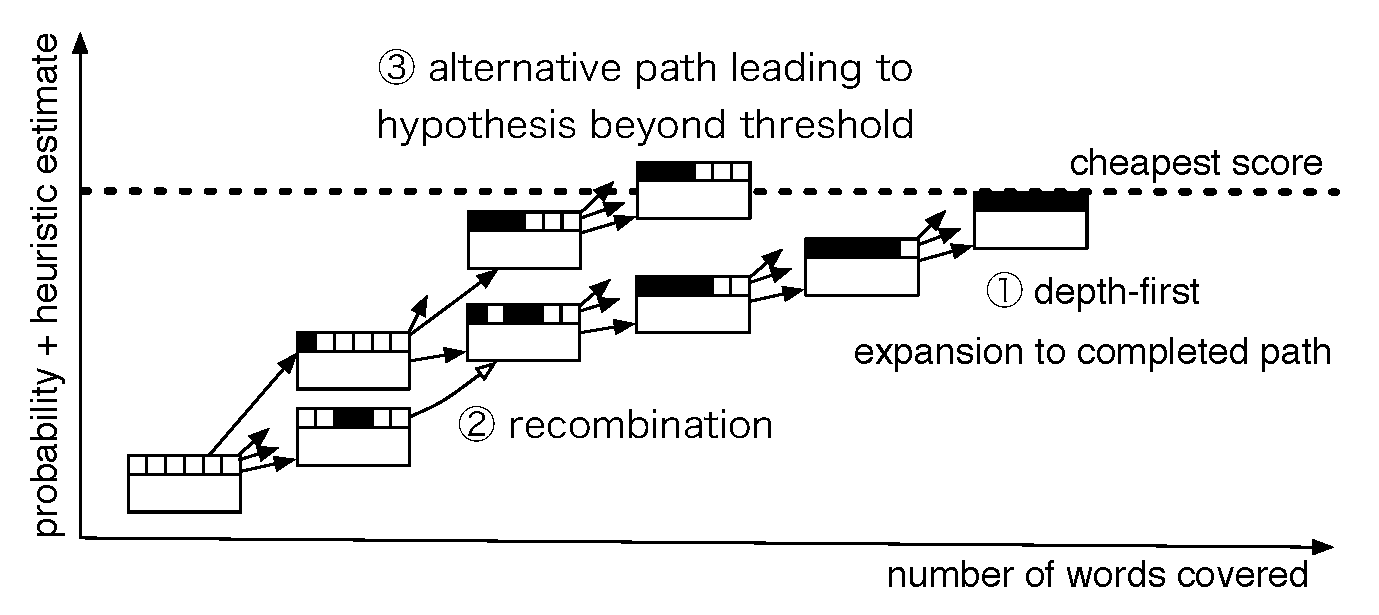
\includegraphics[scale=1]{a-star-search.pdf}
\end{center}
\begin{itemize}\vspace{-5mm}
\item Uses {\em admissible} future cost heuristic: never overestimates cost \vspace{-5mm}
\item Translation agenda: create hypothesis with lowest score + heuristic cost \vspace{-5mm}
\item Done, when complete hypothesis created
\end{itemize}


%%%%%%%%%%%%%%%%%%%%%%%%%%%%%%%%%%%%%%%%%%%%%%%%%%%%%%%%%%%%%%%%%%%%%%%%%%%%

\slide{Greedy Hill-Climbing}
\begin{itemize} \vspace{10mm}
\item Create one complete hypothesis with depth-first search (or other means)
\item Search for better hypotheses by applying change operators
\begin{itemize}
\item change the translation of a word or phrase
\item combine the translation of two words into a phrase
\item split up the translation of a phrase into two smaller phrase translations
\item move parts of the output into a different position
\item swap parts of the output with the output at a different part of the sentence
\end{itemize}
\item Terminates if no operator application produces a better translation
\end{itemize}

%%%%%%%%%%%%%%%%%%%%%%%%%%%%%%%%%%%%%%%%%%%%%%%%%%%%%%%%%%%%%%%%%%%%%%%%%%%%

\slide{Summary}
\begin{itemize} \vspace{10mm}
\item Translation process: produce output left to right
\item Translation options
\item Decoding by hypothesis expansion
\item Reducing search space
\begin{itemize}
\item recombination
\item pruning (requires future cost estimate)
\end{itemize}
\item Other decoding algorithms
\end{itemize}

%%%%%%%%%%%%%%%%%%%%%%%%%%%%%%%%%%%%%%%%%%%%%%%%%%%%%%%%%%%%%%%%%%%%%%%%%%%%


\end{document}
